\chapter{Tensor Calculus, Connections, and Geodesics}

\lectureoverview{Tensor algebra tells us how components transform. Tensor
calculus must do something harder: compare fields at neighboring points
without confusing a change of the field with a change of the coordinate
basis. We will see the ordinary derivative fail, repair it with a
connection, determine the Levi--Civita connection from the metric, and use
it to define geodesics.}

\section{Why Tensor Equations Matter}

Compatible tensors may be added and subtracted, but their index structures
must match. A covector cannot be added directly to a vector, and a
two-index tensor cannot be added to a three-index tensor. This is more than
bookkeeping: each index records one factor in the coordinate
transformation law.

The reason for organizing physics this way is that geometry exists before
coordinates are chosen. A surface may be curved, a mountain may rise from
it, and two points may have a definite separation even if no latitude or
longitude has been assigned. Coordinates become indispensable when we
want numbers and calculations. Tensors let us introduce those numbers
without making the truth of an equation depend on the labels.

For example, a covector transforms according to
\begin{equation}
  V_m^{(y)}
  =
  \frac{\partial x^r}{\partial y^m}V_r^{(x)},
  \label{eq:l05-covector-transform}
\end{equation}
and a mixed tensor according to
\begin{equation}
  \bigl(T^m{}_{n}\bigr)_{(y)}
  =
  \frac{\partial y^m}{\partial x^r}
  \frac{\partial x^s}{\partial y^n}
  \bigl(T^r{}_{s}\bigr)_{(x)}.
  \label{eq:l05-mixed-transform}
\end{equation}
If every component on the right vanishes, every component on the left
vanishes. Thus a tensor equation such as
\begin{equation}
  T^m{}_{n}=0
\end{equation}
is either true in every coordinate system or false in every coordinate
system. The same is true of an equality between tensors with matching
indices.

\begin{figure}[tbp]
  \centering
  
\includegraphics[width=0.86\textwidth]{lecture_05_figure_01.png}
  \caption{Transformation laws make the zero tensor coordinate
  independent. The board displays covariant and mixed examples before the
  lecture turns from tensor algebra to tensor calculus.}
  \lectureframe{00:09:28}
\end{figure}

General relativity needs differential equations, not only algebraic
relations. We therefore need a derivative of a tensor that is again a
tensor. The ordinary partial derivative succeeds for scalars and fails for
vectors; understanding that failure is the central problem of this
lecture.

\section{The Scalar Control Case}

A scalar field assigns one number to each point. Under a coordinate change
the number is unchanged:
\begin{equation}
  \phi^{(y)}(y)=\phi^{(x)}(x).
\end{equation}
The chain rule gives
\begin{equation}
  \frac{\partial\phi}{\partial y^n}
  =
  \frac{\partial x^m}{\partial y^n}
  \frac{\partial\phi}{\partial x^m}.
  \label{eq:l05-scalar-gradient}
\end{equation}
This is precisely the transformation law for a covector. The gradient of
a scalar is therefore a tensor.

\begin{figure}[tbp]
  \centering
  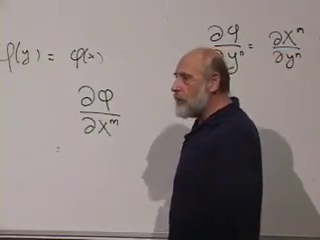
\includegraphics[width=0.82\textwidth]{lecture_05_figure_02.png}
  \caption{The scalar chain rule. The gradient acquires one inverse
  Jacobian and hence one lower index.}
  \lectureframe{00:13:53}
\end{figure}

The physical content is equally simple. If the temperature is constant
throughout a room, all of its derivatives vanish in Cartesian
coordinates. Changing to polar, spherical, or any other smooth
coordinates cannot make the temperature vary. Equation
\eqref{eq:l05-scalar-gradient} guarantees exactly that.

\section{A Constant Vector in a Moving Frame}

Now consider a vector field in an ordinary flat plane. Suppose every arrow
has the same magnitude and points in the same geometric direction. In
Cartesian coordinates its components are constant:
\begin{equation}
  \frac{\partial V_m^{(x)}}{\partial x^n}=0.
  \label{eq:l05-cartesian-constant}
\end{equation}

Lay a curvilinear grid over the same plane. The field has not changed, but
the coordinate directions turn from point to point. Components are
projections onto those local directions, so the \(y\)-components generally
change:
\begin{equation}
  \frac{\partial V_m^{(y)}}{\partial y^n}\neq 0.
  \label{eq:l05-curvilinear-components}
\end{equation}

\begin{figure}[tbp]
  \centering
  
\includegraphics[width=0.86\textwidth]{lecture_05_figure_03.png}
  \caption{One geometrically constant vector field viewed through straight
  and curving coordinate grids. The components change because the local
  axes change.}
  \lectureframe{00:20:35}
\end{figure}

\begin{classroomqa}
\audiencequestion{Does saying that the vector has one fixed direction
already assume some third reference frame common to both coordinate
systems?
\lecturetimestamp{00:18:28--00:20:17}}
\lecturerresponse{The statement is geometric. In the flat plane we may
compare arrows directly, independently of either curvilinear description.
Cartesian coordinates make that comparison especially transparent, but
the vector field does not acquire its direction from the coordinates. The
coordinates only supply components.}
\end{classroomqa}

This example identifies the difficulty. The ordinary derivative of vector
components measures two effects at once: variation of the vector and
variation of the basis. A tensorial derivative must remove the second
effect.

\section{The Ordinary Derivative Fails the Tensor Test}

Let the \(x\)-coordinates be Cartesian for the moment and define
\begin{equation}
  T_{mn}^{(x)}
  \stackrel{?}{=}
  \frac{\partial V_m^{(x)}}{\partial x^n}.
  \label{eq:l05-tentative-tensor}
\end{equation}
If this were a genuine rank-two covariant tensor, its \(y\)-components
would have to be
\begin{align}
  T_{mn}^{(y)}
  &=
  \frac{\partial x^r}{\partial y^m}
  \frac{\partial x^s}{\partial y^n}
  T_{rs}^{(x)}
  \nonumber\\
  &=
  \frac{\partial x^r}{\partial y^m}
  \frac{\partial x^s}{\partial y^n}
  \frac{\partial V_r^{(x)}}{\partial x^s}
  \nonumber\\
  &=
  \frac{\partial x^r}{\partial y^m}
  \frac{\partial V_r^{(x)}}{\partial y^n}.
  \label{eq:l05-expected-transform}
\end{align}

\begin{figure}[tbp]
  \centering
  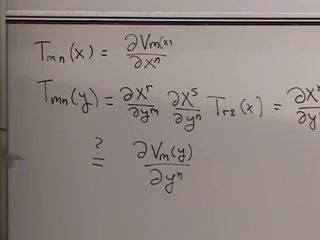
\includegraphics[width=0.88\textwidth]{lecture_05_figure_04.png}
  \caption{The tentative tensor law for
  \(T_{mn}=\partial_n V_m\). The question mark is essential: this is the
  hypothesis being tested, not yet an identity.}
  \lectureframe{00:26:45}
\end{figure}

Now calculate the ordinary derivative of the transformed covector
directly. From Eq.~\eqref{eq:l05-covector-transform},
\begin{align}
  \frac{\partial V_m^{(y)}}{\partial y^n}
  &=
  \frac{\partial}{\partial y^n}
  \left(
    \frac{\partial x^r}{\partial y^m}V_r^{(x)}
  \right)
  \nonumber\\
  &=
  \frac{\partial x^r}{\partial y^m}
  \frac{\partial V_r^{(x)}}{\partial y^n}
  +
  \frac{\partial^2 x^r}
       {\partial y^n\partial y^m}
  V_r^{(x)}.
  \label{eq:l05-product-rule}
\end{align}
The first term is Eq.~\eqref{eq:l05-expected-transform}. The second term is
new. It comes from differentiating the Jacobian that describes the moving
coordinate basis.

\begin{figure}[tbp]
  \centering
  
\includegraphics[width=0.90\textwidth]{lecture_05_figure_05.png}
  \caption{The product rule exposes the extra second-derivative term. This
  term vanishes for a linear coordinate transformation but not for a
  general curvilinear one.}
  \lectureframe{00:32:50}
\end{figure}

\begin{classroomqa}
\audiencequestion{Has the derivative of the Jacobian already been counted
inside the chain-rule term?
\lecturetimestamp{00:31:34--00:32:29}}
\lecturerresponse{No. The chain-rule term differentiates the vector
components while holding the Jacobian factor outside. Directly
differentiating their product also differentiates the Jacobian. That
second derivative of the coordinate map is the missing term, and it is
exactly why the two expressions are unequal.}
\end{classroomqa}

Thus
\begin{equation}
  \frac{\partial V_m^{(y)}}{\partial y^n}
  \neq
  \frac{\partial x^r}{\partial y^m}
  \frac{\partial x^s}{\partial y^n}
  \frac{\partial V_r^{(x)}}{\partial x^s}
\end{equation}
for a general coordinate transformation.

\begin{figure}[tbp]
  \centering
  
\includegraphics[width=0.88\textwidth]{lecture_05_figure_06.png}
  \caption{The completed comparison: the extra product-rule term prevents
  the ordinary component derivative from being a tensor.}
  \lectureframe{00:37:40}
\end{figure}

\begin{classroomqa}
\audiencequestion{Can this failure be seen in a physical field, such as an
electric field?
\lecturetimestamp{00:33:58--00:34:47}}
\lecturerresponse{Yes. A uniform electric field has constant Cartesian
components. In curvilinear coordinates the same field generally has
position-dependent components because the coordinate axes rotate. The
ordinary derivatives then report a change even though the physical field
is uniform.}
\end{classroomqa}

For a linear transformation the Jacobian is constant, so the extra term
vanishes. That special case explains why ordinary component derivatives
behave harmlessly under rotations and other rigid linear changes, while
general coordinate transformations reveal the problem.

\section{From the Extra Term to the Connection}

The failure suggests its own cure. We seek a correction linear in the
vector,
\begin{equation}
  \partial_n V_m + C^r{}_{nm}V_r,
  \label{eq:l05-temporary-connection}
\end{equation}
whose inhomogeneous transformation cancels the derivative of the
Jacobian. The board initially denotes this temporary coefficient by
\(\Gamma\) and writes it with a plus sign for a lower index.

\begin{figure}[tbp]
  \centering
  
\includegraphics[width=0.84\textwidth]{lecture_05_figure_07.png}
  \caption{The first corrected derivative on the board. To keep the later
  Christoffel formula conventional, we denote the temporary plus-sign
  coefficient here by \(C^r{}_{nm}=-\Gamma^r{}_{nm}\).}
  \lectureframe{00:40:30}
\end{figure}

We now adopt the standard Levi--Civita sign convention by defining
\begin{equation}
  C^r{}_{nm}=-\Gamma^r{}_{nm}.
\end{equation}
The covariant derivative of a covector is therefore
\begin{equation}
  \boxed{
  \nabla_n V_m
  =
  \partial_n V_m
  -
  \Gamma^r{}_{nm}V_r.}
  \label{eq:l05-covector-derivative}
\end{equation}
This one normalization resolves the apparent sign change between the early
board equations and the conventional Christoffel formula written later.
No geometry changes; only the name assigned to the temporary correction
coefficient changes.

\begin{classroomqa}
\audiencequestion{Was the correction obtained only because the starting
\(x\)-coordinates were Cartesian, or does a connection exist in a general
geometry?
\lecturetimestamp{00:42:09--00:42:53}}
\lecturerresponse{The Cartesian calculation is the cleanest way to expose
the inhomogeneous term. A connection is defined in general coordinates and
on curved spaces as well. For the metric geometry used here, the metric
will determine the unique torsion-free, metric-compatible connection.}
\end{classroomqa}

The word \emph{covariant} in \emph{covariant derivative} describes the
coordinate-respecting operation. It does not mean that the differentiated
object must carry a lower index.

\subsection{One correction for each index}

Each tensor index contributes its own connection term. With the standard
sign convention, every lower index contributes a minus sign and every
upper index contributes a plus sign. For a rank-two covariant tensor,
\begin{equation}
  \boxed{
  \nabla_p T_{mn}
  =
  \partial_p T_{mn}
  -
  \Gamma^r{}_{pm}T_{rn}
  -
  \Gamma^r{}_{pn}T_{mr}.}
  \label{eq:l05-rank-two-derivative}
\end{equation}

\begin{figure}[tbp]
  \centering
  
\includegraphics[width=0.90\textwidth]{lecture_05_figure_08.png}
  \caption{The board builds the rank-two rule one index at a time using
  the temporary \(C=-\Gamma\) convention. In standard notation the two
  lower-index corrections carry minus signs, as in
  Eq.~\eqref{eq:l05-rank-two-derivative}.}
  \lectureframe{00:49:45}
\end{figure}

The lecture's practical method is useful. Temporarily ignore all but one
tensor index, apply the vector rule to that slot, and then repeat for every
other slot. What must never change is the identity of the free indices.

\begin{classroomqa}
\audiencequestion{Which tensor index belongs in each correction term?
\lecturetimestamp{00:46:14--00:53:21}}
\lecturerresponse{The connection acts on one slot at a time. Acting on the
\(m\)-slot replaces \(m\) by the dummy index \(r\), producing
\(\Gamma^r{}_{pm}T_{rn}\). Acting on the \(n\)-slot produces
\(\Gamma^r{}_{pn}T_{mr}\). The classroom corrections to the board are
important: \(T_{rn}\) and \(T_{mr}\) cannot be interchanged without an
independent symmetry.}
\end{classroomqa}

\begin{classroomqa}
\audiencequestion{May a free index be swapped with a repeated index?
\lecturetimestamp{00:53:55--00:54:51}}
\lecturerresponse{No. A repeated index is a dummy summation label and may
be renamed consistently within its term. A free index identifies a
component of the result and must remain free in the same position in every
term. Indices may be interchanged only when a stated symmetry permits it.}
\end{classroomqa}

For a vector with an upper index,
\begin{equation}
  \boxed{
  \nabla_m V^n
  =
  \partial_m V^n
  +
  \Gamma^n{}_{mr}V^r.}
  \label{eq:l05-vector-derivative}
\end{equation}
A scalar has no tensor index on which the connection can act, so
\(\nabla_m\phi=\partial_m\phi\).

\section{The Polar-Coordinate Test}

The abstract rule becomes visible in polar coordinates. On the flat plane,
\begin{equation}
  ds^2=dr^2+r^2d\theta^2,
  \qquad
  g_{rr}=1,
  \qquad
  g_{\theta\theta}=r^2.
  \label{eq:l05-polar-metric}
\end{equation}
Ignore the singular origin and consider the radial field
\begin{equation}
  V^r=1,
  \qquad
  V^\theta=0.
  \label{eq:l05-radial-field}
\end{equation}
Its polar components are constant, yet the arrows point in different
Cartesian directions around the origin. The field is not geometrically
constant.

\begin{figure}[tbp]
  \centering
  
\includegraphics[width=0.80\textwidth]{lecture_05_figure_09.png}
  \caption{The radial field has constant polar components
  \(V^r=1\), \(V^\theta=0\), but its direction changes from point to point.}
  \lectureframe{00:56:52}
\end{figure}

The nonzero polar Christoffel symbols are
\begin{equation}
  \Gamma^r{}_{\theta\theta}=-r,
  \qquad
  \Gamma^\theta{}_{r\theta}
  =
  \Gamma^\theta{}_{\theta r}
  =
  \frac{1}{r}.
  \label{eq:l05-polar-christoffel}
\end{equation}
Consequently,
\begin{equation}
  \nabla_\theta V^\theta
  =
  \Gamma^\theta{}_{\theta r}V^r
  =
  \frac{1}{r}\neq 0.
\end{equation}
The covariant derivative detects the turning of the field even though the
ordinary derivatives of its polar components vanish.

\begin{classroomqa}
\audiencequestion{Does Cartesian simply mean that the coordinate lines
look straight, as on a Mercator map?
\lecturetimestamp{00:59:32--01:00:30}}
\lecturerresponse{No. Here Cartesian means that the flat-space metric has
constant components \(g_{mn}=\delta_{mn}\). A drawing may use straight
grid lines while distorting the metric. Conversely, polar coordinates
describe a flat plane even though their coordinate basis changes from
point to point.}
\end{classroomqa}

\section{Metric Compatibility}

The connection has so far been introduced as the correction needed for
tensorial differentiation. We now determine it from the metric. In flat
Cartesian coordinates the metric is constant, so its covariant derivative
should vanish. Since \(\nabla_p g_{mn}\) is a tensor, vanishing in those
coordinates implies vanishing in every coordinate system:
\begin{equation}
  \boxed{\nabla_p g_{mn}=0.}
  \label{eq:l05-metric-compatibility}
\end{equation}
Using the standard convention,
\begin{equation}
  0
  =
  \partial_p g_{mn}
  -
  \Gamma^r{}_{pm}g_{rn}
  -
  \Gamma^r{}_{pn}g_{mr}.
  \label{eq:l05-metric-compatibility-expanded}
\end{equation}

\begin{figure}[tbp]
  \centering
  
\includegraphics[width=0.90\textwidth]{lecture_05_figure_10.png}
  \caption{Metric compatibility expanded on the board in the temporary
  \(C=-\Gamma\) notation. Converting to the standard Christoffel symbol
  yields Eq.~\eqref{eq:l05-metric-compatibility-expanded}.}
  \lectureframe{01:03:30}
\end{figure}

\begin{classroomqa}
\audiencequestion{Why choose the covariant derivative of the metric to be
zero?
\lecturetimestamp{01:18:26--01:19:49}}
\lecturerresponse{In homogeneous flat space the metric is the same at every
point in Cartesian coordinates, so its ordinary derivative vanishes.
The covariant derivative is designed to preserve that geometric statement
in arbitrary coordinates. More deeply, \(\nabla g=0\) says that parallel
transport preserves lengths and angles.}
\end{classroomqa}

Metric compatibility alone leaves the possibility of torsion. The
connection used here is also taken to be torsion-free,
\begin{equation}
  \Gamma^a{}_{bc}=\Gamma^a{}_{cb}.
\end{equation}
These two conditions determine the Levi--Civita connection uniquely.
Permuting the indices in
Eq.~\eqref{eq:l05-metric-compatibility-expanded}, adding two equations,
subtracting the third, and raising one index gives
\begin{equation}
  \boxed{
  \Gamma^a{}_{bc}
  =
  \frac{1}{2}g^{ad}
  \left(
    \partial_b g_{dc}
    +
    \partial_c g_{db}
    -
    \partial_d g_{bc}
  \right).}
  \label{eq:l05-christoffel}
\end{equation}

\begin{figure}[tbp]
  \centering
  
\includegraphics[width=0.91\textwidth]{lecture_05_figure_11.png}
  \caption{The conventional Christoffel formula. Its lower indices
  \(b,c\) are symmetric, and the upper index is produced by the inverse
  metric \(g^{ad}\).}
  \lectureframe{01:09:43}
\end{figure}

The Christoffel symbols are also called connection coefficients or an
affine connection. They are built from the metric and its first
derivatives. They are not themselves the components of a tensor.

\begin{classroomqa}
\audiencequestion{Are there two kinds of Christoffel symbol, and may their
indices be raised and lowered with the metric?
\lecturetimestamp{01:05:34--01:07:46}}
\lecturerresponse{One often writes both
\(\Gamma^a{}_{bc}\) and
\(\Gamma_{abc}=g_{ad}\Gamma^d{}_{bc}\). They are related by the metric, but
the connection is not a tensor, so this notation must not be mistaken for
an ordinary tensor transformation law. The Levi--Civita formula makes the
relationship well defined in the chosen coordinates.}
\end{classroomqa}

\begin{classroomqa}
\audiencequestion{Should the derivatives in the Christoffel formula use
\(x\) or \(y\) coordinates?
\lecturetimestamp{01:09:39--01:10:15}}
\lecturerresponse{Use whichever coordinate system supplies the metric
components. If the metric is written as \(g_{mn}(y)\), differentiate with
respect to \(y\); the resulting numbers are the connection coefficients
in the \(y\)-coordinates.}
\end{classroomqa}

\begin{classroomqa}
\audiencequestion{If all three indices are lowered, is the result symmetric
in all three?
\lecturetimestamp{01:13:17--01:15:13}}
\lecturerresponse{No. For the torsion-free Levi--Civita connection,
\(\Gamma^a{}_{bc}\) is symmetric only in \(b\) and \(c\). Lowering \(a\)
does not create symmetry with that slot; the minus sign in
Eq.~\eqref{eq:l05-christoffel} already distinguishes it.}
\end{classroomqa}

The same connection acts on upper-index components with the opposite sign
from lower-index components, as in
Eq.~\eqref{eq:l05-vector-derivative}.

\begin{figure}[tbp]
  \centering
  
\includegraphics[width=0.88\textwidth]{lecture_05_figure_12.png}
  \caption{Covariant differentiation of an upper-index vector. In the
  standard convention the connection term enters with a plus sign.}
  \lectureframe{01:13:15}
\end{figure}

\begin{classroomqa}
\audiencequestion{Can the metric be used to lower an index on something
that is not a tensor?
\lecturetimestamp{01:15:38--01:17:23}}
\lecturerresponse{For this metric-derived connection, the lowered
coefficient is a useful and consistent abbreviation. But the result does
not thereby become a tensor. Index lowering preserves tensorial character
when one starts with a tensor; it cannot manufacture tensorial
transformation behavior from a connection coefficient.}
\end{classroomqa}

In \(D\) dimensions there are \(D^3\) displayed connection coefficients:
27 in three dimensions and 64 in four. Symmetry in the two lower indices
reduces the number of independent coefficients, but practical
calculations can still be lengthy. The point of the construction is the
logic: the connection terms convert ordinary component differentiation
into a geometric operation.

\section{What the Connection Means Locally}

The fact that \(\Gamma^a{}_{bc}\) is not a tensor can be seen immediately.
In flat Cartesian coordinates the metric is constant, so all Christoffel
symbols vanish. In polar coordinates on the same flat plane they do not
vanish. A tensor that vanished in one coordinate system would vanish in
all of them.

The transformation law contains an inhomogeneous second-derivative term:
\begin{align}
  \Gamma'^a{}_{bc}
  &=
  \frac{\partial y^a}{\partial x^r}
  \frac{\partial x^m}{\partial y^b}
  \frac{\partial x^n}{\partial y^c}
  \Gamma^r{}_{mn}
  \nonumber\\
  &\quad+
  \frac{\partial y^a}{\partial x^r}
  \frac{\partial^2 x^r}
       {\partial y^b\partial y^c}.
  \label{eq:l05-connection-transform}
\end{align}
That inhomogeneous term is not a defect. It is exactly what cancels the
corresponding term from differentiating tensor components.

\begin{classroomqa}
\audiencequestion{Is there a coordinate-free way to understand the
covariant derivative?
\lecturetimestamp{01:19:51--01:23:55}}
\lecturerresponse{At any chosen point \(p\), one may introduce normal
coordinates for which
\[
  g_{mn}(p)=\delta_{mn}
  \quad\text{and}\quad
  \partial_r g_{mn}(p)=0
\]
in a Riemannian space, with the corresponding Minkowski metric in
spacetime. Hence \(\Gamma^a{}_{bc}(p)=0\), and at that point the covariant
derivative equals the ordinary derivative. The construction compares
nearby tensors as they would be compared in the locally flattened frame.
Only the statement at the chosen point is exact; curvature remains in
second derivatives and prevents one normal frame from flattening an
extended curved region.}
\end{classroomqa}

\begin{figure}[tbp]
  \centering
  
\includegraphics[width=0.88\textwidth]{lecture_05_figure_13.png}
  \caption{Locally Cartesian coordinates at one point of a curved surface.
  The metric and its first derivatives can be normalized there even when
  no single coordinate system flattens the whole surface.}
  \lectureframe{01:21:45}
\end{figure}

\begin{classroomqa}
\audiencequestion{If the Christoffel symbols are zero, is that the
definition of flat space?
\lecturetimestamp{01:23:56--01:25:59}}
\lecturerresponse{Not at a single point. Normal coordinates can make them
zero at any chosen point even in curved space. Flatness means that one can
find coordinates in which they vanish throughout a neighborhood, or
equivalently that the curvature tensor vanishes there. Conversely,
curvilinear coordinates can make the Christoffel symbols nonzero even in
flat space. In polar coordinates it is
\(g_{\theta\theta}=r^2\), not \(g_{rr}\), that varies with \(r\).}
\end{classroomqa}

\begin{classroomqa}
\audiencequestion{Is the exterior derivative the same operation?
\lecturetimestamp{01:26:02--01:26:58}}
\lecturerresponse{No. The exterior derivative acts on differential forms
and is tensorial without a connection. In three Euclidean dimensions, the
exterior derivative of a one-form corresponds, after applying the Hodge
dual, to the familiar curl. That is a related but distinct construction
and is deferred here.}
\end{classroomqa}

\section{Differentiation Along a Curve}

Let a curve be described by coordinates \(y^m(s)\), where \(s\) is arc
length. Its tangent vector is
\begin{equation}
  t^m
  =
  \frac{dy^m}{ds},
  \qquad
  g_{mn}t^m t^n=1.
  \label{eq:l05-tangent}
\end{equation}

\begin{figure}[tbp]
  \centering
  
\includegraphics[width=0.80\textwidth]{lecture_05_figure_14.png}
  \caption{A curve parameterized by arc length \(s\), with the tangent
  direction marked along the path.}
  \lectureframe{01:29:10}
\end{figure}

For a scalar field, differentiation along the curve is an ordinary chain
rule:
\begin{equation}
  \frac{d\phi}{ds}
  =
  \frac{\partial\phi}{\partial y^m}
  \frac{dy^m}{ds}
  =
  t^m\partial_m\phi.
  \label{eq:l05-scalar-path}
\end{equation}

\begin{figure}[tbp]
  \centering
  
\includegraphics[width=0.88\textwidth]{lecture_05_figure_15.png}
  \caption{The derivative of a scalar along a curve is the contraction of
  its gradient with the tangent vector.}
  \lectureframe{01:30:30}
\end{figure}

\begin{classroomqa}
\audiencequestion{Is \(dy^m/ds\) the slope, and why does it have unit
length?
\lecturetimestamp{01:30:33--01:31:49}}
\lecturerresponse{It is the tangent vector rather than a single coordinate
slope. A slope such as \(dy/dx\) compares two coordinates; \(dy^m/ds\)
lists all components of the tangent. Because \(s\) is arc length,
\(g_{mn}(dy^m/ds)(dy^n/ds)=1\).}
\end{classroomqa}

For a vector, the ordinary derivative along the curve is still not
tensorial. We first take the covariant derivative and then contract its
derivative index with the tangent:
\begin{equation}
  \boxed{
  \frac{D V^n}{Ds}
  \equiv
  t^m\nabla_m V^n.}
  \label{eq:l05-path-derivative-definition}
\end{equation}

\begin{figure}[tbp]
  \centering
  
\includegraphics[width=0.88\textwidth]{lecture_05_figure_16.png}
  \caption{The pathwise covariant derivative is obtained by contracting
  the ordinary covariant derivative with the tangent direction.}
  \lectureframe{01:36:30}
\end{figure}

Expanding the definition,
\begin{align}
  \frac{D V^n}{Ds}
  &=
  \left(
    \partial_m V^n
    +
    \Gamma^n{}_{mr}V^r
  \right)
  \frac{dy^m}{ds}
  \nonumber\\
  &=
  \frac{dV^n}{ds}
  +
  \Gamma^n{}_{mr}V^r\frac{dy^m}{ds}.
  \label{eq:l05-path-derivative-expanded}
\end{align}

\begin{figure}[tbp]
  \centering
  
\includegraphics[width=0.90\textwidth]{lecture_05_figure_17.png}
  \caption{The expanded path derivative: ordinary change of the vector
  components plus the connection correction along the tangent.}
  \lectureframe{01:39:15}
\end{figure}

\begin{classroomqa}
\audiencequestion{Are the coordinates along this curve assumed to be
Cartesian?
\lecturetimestamp{01:34:26--01:34:49}}
\lecturerresponse{No. The point of
Eq.~\eqref{eq:l05-path-derivative-expanded} is that it works in arbitrary
coordinates. In Cartesian coordinates on flat space the Christoffel
symbols vanish and the familiar ordinary derivative is recovered.}
\end{classroomqa}

\section{Geodesics}

Now differentiate the tangent vector itself. Set
\begin{equation}
  V^n=t^n=\frac{dy^n}{ds}.
\end{equation}
Then
\begin{equation}
  \frac{D t^n}{Ds}
  =
  \frac{d^2y^n}{ds^2}
  +
  \Gamma^n{}_{mr}
  \frac{dy^m}{ds}
  \frac{dy^r}{ds}.
  \label{eq:l05-tangent-derivative}
\end{equation}
In flat Cartesian coordinates, this vanishes along a straight line because
the tangent is constant. The tensorial form lets us use the same criterion
in curvilinear coordinates and in genuinely curved spaces.

\begin{definition}
A geodesic is an affinely parameterized curve whose tangent vector is
covariantly constant:
\begin{equation}
  \boxed{
  \frac{D t^n}{Ds}=0.}
  \label{eq:l05-geodesic-definition}
\end{equation}
Equivalently,
\begin{equation}
  \boxed{
  \frac{d^2y^n}{ds^2}
  +
  \Gamma^n{}_{mr}
  \frac{dy^m}{ds}
  \frac{dy^r}{ds}
  =
  0.}
  \label{eq:l05-geodesic-equation}
\end{equation}
\end{definition}

\begin{figure}[tbp]
  \centering
  
\includegraphics[width=0.90\textwidth]{lecture_05_figure_18.png}
  \caption{The geodesic equation on the board. A geodesic is the curve
  whose tangent transports itself without turning relative to the
  connection.}
  \lectureframe{01:44:45}
\end{figure}

In flat space the geodesics are straight lines. In a curved space they are
the straightest available curves: their tangent vectors are parallel
transported along themselves. This condition can hold even though no
coordinate system makes the whole space flat.

\begin{classroomqa}
\audiencequestion{Could one use a contravariant derivative instead of the
covariant derivative in the definition?
\lecturetimestamp{01:46:19--01:47:11}}
\lecturerresponse{The terminology is causing the confusion.
\emph{Covariant derivative} names the coordinate-covariant operation; here
it is acting on the contravariant tangent \(t^n\). Lowering the tangent
with the metric gives the equivalent lower-index equation because the
Levi--Civita connection satisfies \(\nabla g=0\).}
\end{classroomqa}

\subsection{The road to gravity}

In special relativity, a force-free particle follows a straight worldline
in flat spacetime. In general relativity, a freely falling particle follows
a spacetime geodesic. With proper time \(\tau\) as affine parameter,
\begin{equation}
  \frac{d^2x^\mu}{d\tau^2}
  =
  -
  \Gamma^\mu{}_{\alpha\beta}
  \frac{dx^\alpha}{d\tau}
  \frac{dx^\beta}{d\tau}.
  \label{eq:l05-spacetime-geodesic}
\end{equation}
The left side resembles acceleration, while the right side contains first
derivatives of the metric through the Christoffel symbols.

\begin{figure}[tbp]
  \centering
  
\includegraphics[width=0.88\textwidth]{lecture_05_figure_19.png}
  \caption{The closing comparison with Newtonian motion. Coordinate
  acceleration is related to a spatial derivative of the gravitational
  potential, while the relativistic geodesic equation contains first
  derivatives of the metric through \(\Gamma\).}
  \lectureframe{01:50:15}
\end{figure}

Newtonian gravity writes
\begin{equation}
  m\frac{d^2\bm{x}}{dt^2}
  =
  -m\bm{\nabla}\Phi,
  \label{eq:l05-newton}
\end{equation}
so the mass cancels. In the weak, slowly varying field limit,
\begin{equation}
  g_{00}
  \simeq
  1+\frac{2\Phi}{c^2},
  \qquad
  \Gamma^i{}_{00}
  \simeq
  \frac{1}{c^2}\partial_i\Phi,
\end{equation}
and the spatial part of
Eq.~\eqref{eq:l05-spacetime-geodesic} reduces to
\begin{equation}
  \frac{d^2x^i}{dt^2}
  \simeq
  -\partial_i\Phi.
\end{equation}
This is only a preview of the derivation, but it makes the destination
clear: what Newtonian language calls gravitational force is encoded in
the spacetime metric and its connection. A freely falling particle feels
no nongravitational proper force; its worldline is straight in the
geometric sense expressed by the geodesic equation.

One concept remains before curvature can be defined operationally:
parallel transport around different paths. Curvature will measure the
obstruction to making those comparisons path independent, and therefore
the obstruction to flattening the geometry beyond a single point.
